\documentclass[aspectratio=169]{beamer}
\usetheme{Madrid}
\usecolortheme{beaver}
\usepackage[utf8]{inputenc}
\usepackage[T1]{fontenc}
\usepackage{tikz}
\usepackage{amssymb}
\usepackage{graphicx}
\setbeamertemplate{navigation symbols}{}
\setbeamercolor{title}{fg=white,bg=cyan!60!black}
\setbeamercolor{frametitle}{fg=white,bg=cyan!50!black}
\setbeamercolor{block title}{bg=cyan!15,fg=black}
\setbeamercolor{block body}{bg=cyan!5,fg=black}

\title{G7 — Game States}
\subtitle{Menu → playing → paused → game-over → win}
\author{ByteForge --- Grade 7 --- Game Maker}
\date{}

\begin{document}

\begin{frame}
    \titlepage
\end{frame}

\begin{frame}{Today's Plan}
    \begin{itemize}
        \item The State Variable
        \item Switching States
        \item Pause Overlay
        \item[$\bigstar$] BOSS --- Full Game Loop w/ Screens
    \end{itemize}
\end{frame}

\begin{frame}{A state is just a variable holding text}
    \Large
    What makes it a "state machine" is using IF/ELSE to draw a completely different screen depending on what the variable currently holds.

    \begin{center}
    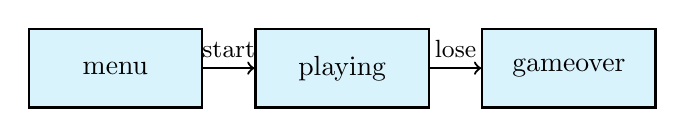
\begin{tikzpicture}[scale=0.9]

        \node[draw, thick, minimum width=2.2cm, minimum height=1cm, fill=cyan!15] (m) at (0,0) {menu};
        \node[draw, thick, minimum width=2.2cm, minimum height=1cm, fill=cyan!15] (p) at (3.2,0) {playing};
        \node[draw, thick, minimum width=2.2cm, minimum height=1cm, fill=cyan!15] (g) at (6.4,0) {gameover};
        \draw[->, thick] (m) -- (p) node[midway, above]{\small start};
        \draw[->, thick] (p) -- (g) node[midway, above]{\small lose};
    \end{tikzpicture}
    \end{center}
\end{frame}


\begin{frame}{A condition that changes the state itself}
    \Large
    The game changes its own state variable based on a condition — this self-modifying behaviour is exactly how real games transition between screens.
\end{frame}


\begin{frame}{A flag that gates everything else}
    \Large
    A true/false "paused" variable draws an overlay on top — whatever you draw LAST appears on top of everything drawn before it.
\end{frame}


\begin{frame}{BOSS — a real, multi-state machine}
    \Large
    menu to playing to gameover, each transition triggered by a real condition — the exact pattern behind every real video game's screen flow.
\end{frame}

\begin{frame}{Real-World Example}
    \Large
    Every app you use has "states": a login screen, a loading spinner, the main screen, an error message — the same menu/playing/paused/gameover idea, just with different names. Minecraft has this too: title screen, world-loading screen, playing, the ESC pause menu, and the respawn/death screen are all states of ONE running program.
\end{frame}


\begin{frame}{Image}
    \begin{center}
    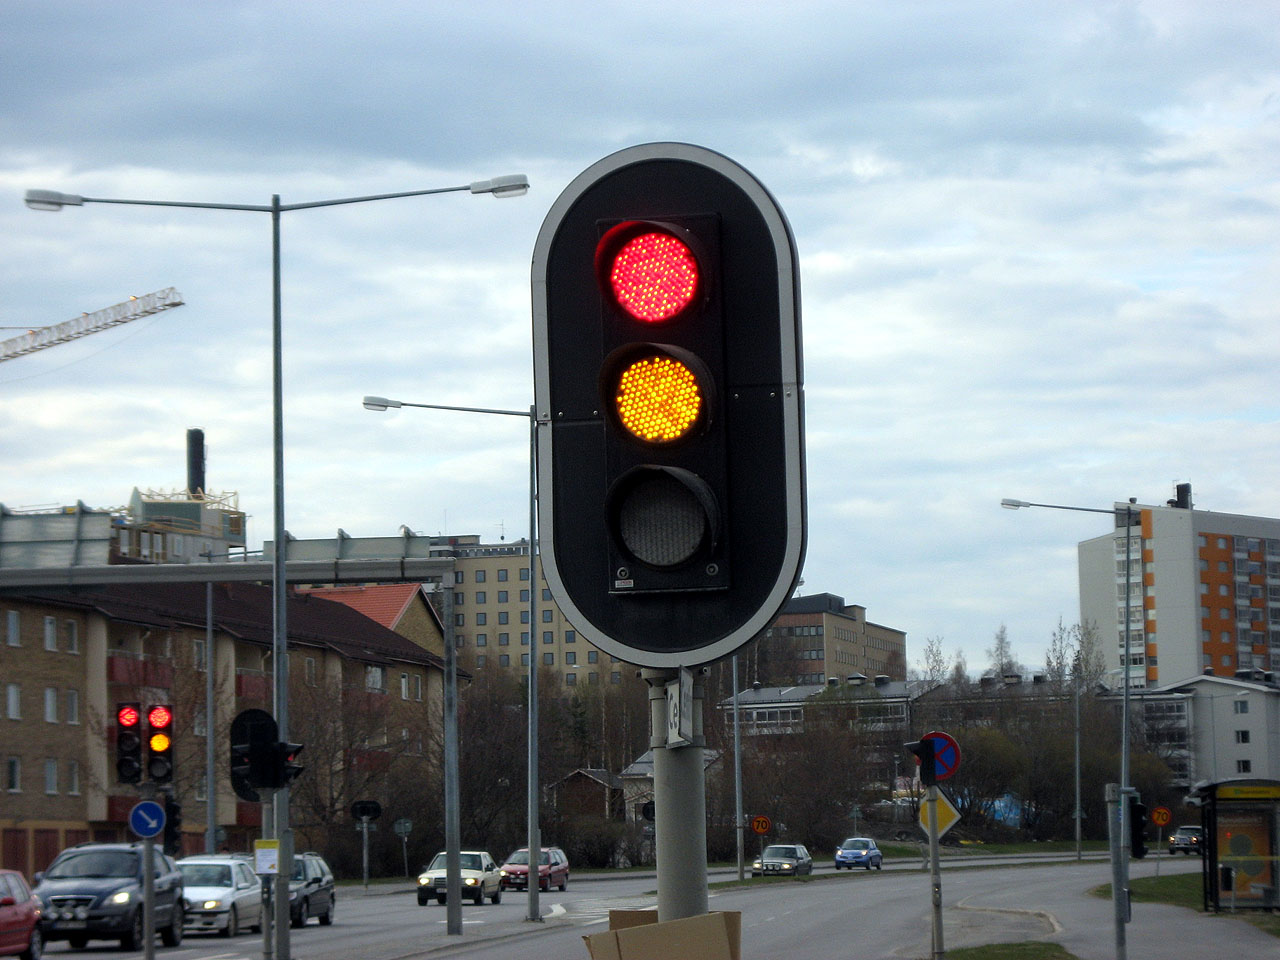
\includegraphics[width=0.5\textwidth]{images/traffic.jpg}

    \large Three distinct states --- red, amber, green --- the same idea as menu/playing/paused.

    \small LED traffic lights, public domain (PD-self), via Wikimedia Commons
    \end{center}
\end{frame}

\begin{frame}{Let Them Discover}
    \Large
    List every distinct "screen" Minecraft (or any game) shows you from opening the app to actually playing (splash screen, menu, loading, playing, pause, death/game over). How many states is that, really?
\end{frame}

\begin{frame}{Your Turn}
    \Large
    Open the student map, find \textbf{G7 — Game States}, and work through it
    hands-on --- everything you just saw, they now do themselves.
\end{frame}

\end{document}
